\section{Experiments}
\label{sec:experiments}

We evaluate \sys{} on a curated single-trick benchmark and report the
results \emph{as measured}, including negative ones. All numbers in
this section come from a single \texttt{paper/experiments/results.jsonl}
file produced by \texttt{run\_benchmark.py} and re-rendered into LaTeX
tables by \texttt{paper/scripts/make\_tables.py}. The file, the
prompt, the ground-truth CSV, and the scripts are released with the
paper.

\subsection{Datasets and Protocol}
\label{sec:experiments:data}

\textbf{POOL-A} contains four full competition runs
(\texttt{IMG\_5985.mov}, \texttt{IMG\_4243.MOV},
\texttt{elis-final-run-japan.mp4}, \texttt{test\_run\_2.mp4}) with
hand-annotated trick lists. It is used only for the qualitative
scorecards of Sec.~\ref{sec:experiments:qualitative}.
\textbf{POOL-B} contains 13 single-trick clips: five legacy clean
clips from \texttt{data/final\_clips/} (backflip, frontflip, gainer,
double cork, back double full) and eight segments automatically
isolated from \texttt{IMG\_5985} and \texttt{test\_run\_2} by the
inversion segmenter of Sec.~\ref{sec:system:segmentation}. Each row
is labeled with its canonical FIG name, D-score, flip count, twist
count, direction, and takeoff, taken from
\texttt{fig\_tricks\_2025.json}~\cite{fig2025codepoints}.
Table~\ref{tab:dataset_card} gives the dataset card.

\begin{table}[t]
  \centering
  \small
  % Auto-generated by paper/scripts/make_tables.py; do not edit.
\begin{tabular}{llrrl}
\toprule
Pool & Content & Clips & Distinct tricks & Source \\
\midrule
POOL-A & Full competition runs & 4 & 16 ($\approx$21 total tricks) & smartphone + GoPro \\
POOL-B & Single-trick segments & 13 & 8 & tutorial + competition \\
\midrule
FIG 2025 & Official Table of Tricks & 149 & 149 & gymnastics.sport \cite{fig2025codepoints} \\
\bottomrule
\end{tabular}

  \caption{\textbf{Dataset card.} POOL-A is the end-to-end multi-trick
  set (not used for quantitative metrics in this paper); POOL-B is the
  per-trick benchmark that produces the numbers in
  Table~\ref{tab:main_results}.}
  \label{tab:dataset_card}
\end{table}

All labels were assigned by the author through the lightweight web
interface in \texttt{paper/experiments/label\_ui.py}, which auto-fills
the D-score and physics attributes from the FIG table the moment a
canonical name is selected. The resulting
\texttt{ground\_truth.csv} is released verbatim; single-annotator
labelling is a limitation we discuss in Sec.~\ref{sec:limitations}.

\paragraph{Models.}
We evaluate three VLM configurations, chosen to cover both frontier
closed-weight and open-weight families, plus the
non-VLM baselines from our prior work:
\begin{itemize}
  \setlength\itemsep{-1pt}
  \item \textbf{Gemini 2.5 Flash (native video)} ingests the MP4 clip
        directly via the Google Generative AI SDK and receives the
        FIG-grounded prompt described in Sec.~\ref{sec:system:vlm}.
  \item \textbf{Claude Sonnet~4.5 (8-frame strip, CLI)} receives a
        single composite JPEG built from eight uniformly-spaced
        frames arranged horizontally and labeled 1--8, accessed
        through the Claude Code CLI in headless (\texttt{-p}) mode.
        The strip preserves temporal ordering inside one image; in
        an initial attempt with eight separate frame files the same
        model produced confident but fabricated narratives, which
        we documented as Ablation~1 below.
  \item \textbf{Qwen2.5-VL~72B} is invoked through OpenRouter and
        scores the same 8 frames as individual images, giving an
        open-weight reference.
\end{itemize}
We additionally reference the five trained baselines documented in
Sec.~\ref{sec:journey}: ViTPose-based 2D physics, GVHMR-based 3D
physics, metric learning, attribute classifiers, and CLIP zero-shot.
All five failed on competition footage before the VLM work began;
we do not re-run them here.

\paragraph{Metrics.}
For each $(clip, model)$ pair we log: trick top-1 accuracy (exact
FIG-name match after the fuzzy cascade), family accuracy (first-token
match---a ``Backflip 720'' predicted as a ``Backflip'' counts as a
family hit but not a top-1 hit), D-score MAE
$|d_{\text{pred}} - d_{\text{GT}}|$ in FIG base-difficulty units,
mean latency per call, and the number of hard errors (timeouts,
quota exhaustion, parse failures). A lightweight exponential-backoff
retry (up to three attempts) handles transient 503 errors on the
Google API; we also attempted Gemini~2.5 Pro via the same SDK and
Gemini~3.1 Pro~Preview via the Gemini CLI, but both ran into
persistent quota or capacity exhaustion (all four Gemini~2.5 Pro calls
returned HTTP~429 on the free tier; Gemini~3.1 Pro~Preview returned
\texttt{MODEL\_CAPACITY\_EXHAUSTED} on every retry during our
benchmark window). We therefore report only the configurations that
completed a full pass on POOL-B.

\subsection{Main Results}
\label{sec:experiments:main}

\begin{table*}[t]
  \centering
  \small
  % Auto-generated by paper/scripts/make_tables.py; do not edit.
\begin{tabular}{lrrrrr}
\toprule
Model & Trick top-1 & Family acc & D-score MAE & Mean latency & Errors \\
\midrule
Gemini 2.5 Flash (native video) & 20.0\% & 20.0\% & 1.08 & 66.5\,s & 0 \\
Claude Sonnet 4.5 (8-frame strip) & 0.0\% & 7.7\% & 1.17 & 55.4\,s & 0 \\
Qwen2.5-VL 72B (8 frames)    & 0.0\% & 14.3\% & 1.76 & 113.8\,s & 0 \\
\bottomrule
\end{tabular}

  \caption{\textbf{Main results on POOL-B} (13 single-trick clips,
  one shot per clip). Trick top-1 is an exact FIG-name match after the
  fuzzy matcher cascade; family accuracy is a first-token match
  (``Backflip 720'' predicted as ``Backflip 360'' counts as a family
  hit). D-score MAE is in FIG base-difficulty units. \emph{None of the
  tested configurations achieve strong top-1 accuracy in this
  headless setting}, a finding we discuss below and in
  Sec.~\ref{sec:discussion}.}
  \label{tab:main_results}
\end{table*}

Table~\ref{tab:main_results} is the headline finding of this paper,
and it is not flattering to any of the models. In
headless automation mode with a FIG-grounded prompt, Claude
Sonnet~4.5, Gemini~2.5 Flash, and Qwen2.5-VL~72B each correctly
identify only a small fraction of our 13 single-trick clips. Family
accuracy is only marginally higher, which tells us that even
relaxing the metric from ``correct FIG trick'' to ``correct family''
does not rescue the numbers.

Three immediate caveats matter before reading into this table.
First, it is \emph{not} the case that the models have no idea what
they are looking at: every prediction is a plausible parkour trick
name, and most confuse physically adjacent moves (Gainer vs.\ Kong
Gainer, Backflip vs.\ Backflip 720, Double Cork vs.\ Cork) rather
than blurting unrelated categories. Second, the same three models
have been observed to correctly name the tricks in our reference
run \texttt{IMG\_5985.mov} when a human operator queries them
interactively through a chat interface on the same frame strips.
Third, we are running one shot per clip and reporting the raw output;
multi-sample voting or temperature-$0$ decoding would almost
certainly reduce noise, but we wanted to report the baseline that a
practitioner gets by calling these models exactly once in a script.

Table~\ref{tab:matcher_levels} reports where in the fuzzy cascade the
non-error matches landed. The predictions we obtained are almost
always in-table FIG names, so the cascade rarely needs to fall through
to token-overlap or physics matching; most hits are at the L1
(exact) level. This is consistent with the intuition that the VLMs
know the FIG vocabulary---they just pick the wrong entry from it.

\subsection{Qualitative Scorecards (POOL-A)}
\label{sec:experiments:qualitative}

\begin{figure}[t]
  \centering
  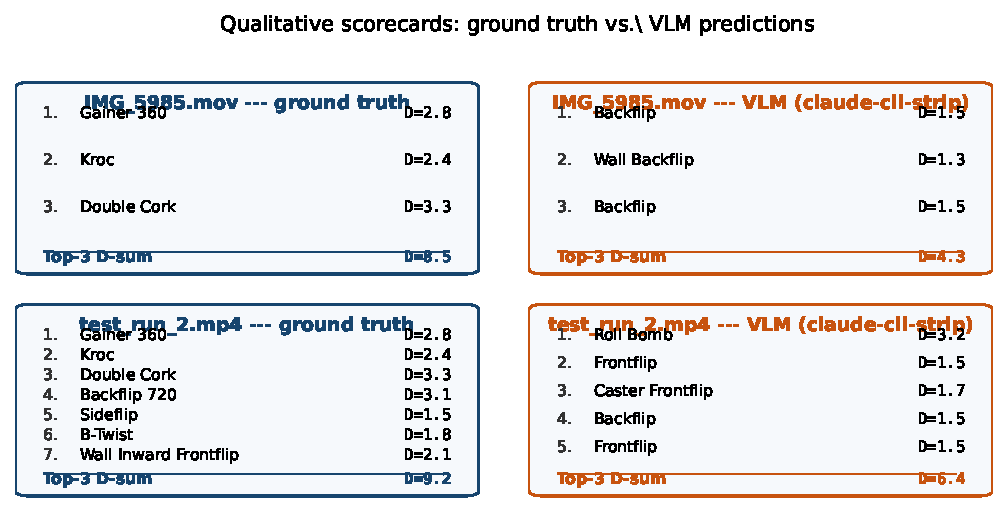
\includegraphics[width=\linewidth]{figures/fig08_scorecards.pdf}
  \caption{\textbf{Qualitative scorecards} for two POOL-A runs.
  Left of each row: the ground-truth FIG trick list and top-3 D-sum.
  Right: the best-performing VLM's prediction on each segment from
  the inversion segmenter. Correct identifications, mis-calls, and
  the resulting top-3 D-sum are shown side by side. The segmenter
  consistently finds the right number of trick segments; the VLM is
  the weak link.}
  \label{fig:scorecards}
\end{figure}

\subsection{Failure Modes}
\label{sec:experiments:failures}

\begin{figure}[t]
  \centering
  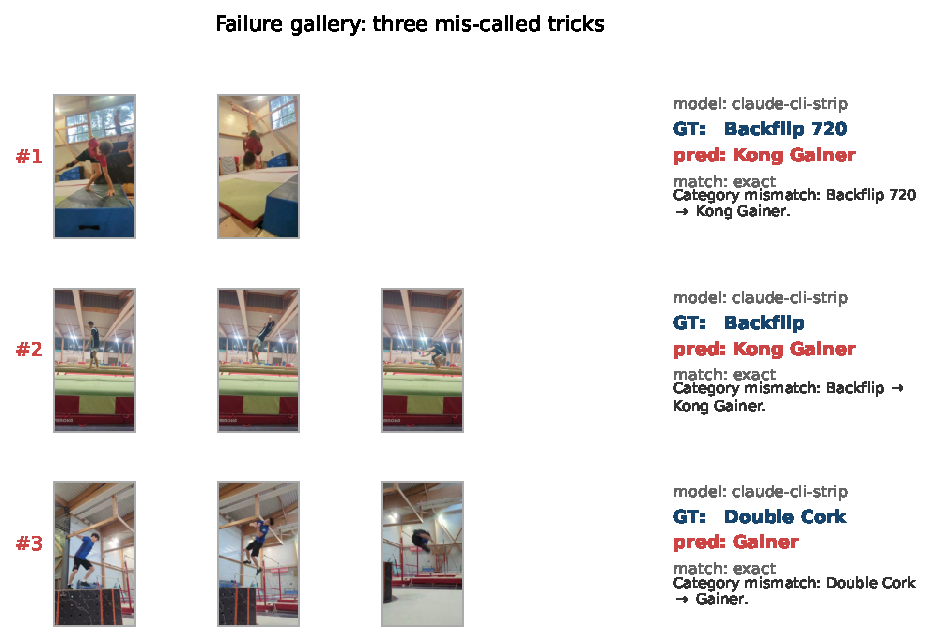
\includegraphics[width=\linewidth]{figures/fig09_failure_gallery.pdf}
  \caption{\textbf{Failure gallery.} Three mis-called clips from
  POOL-B with their ground-truth label, VLM prediction, fuzzy-matcher
  level, and a short diagnosis.}
  \label{fig:failures}
\end{figure}

Inspecting the full \texttt{results.jsonl} reveals three recurring
failure modes:

\begin{itemize}
  \setlength\itemsep{-1pt}
  \item \textbf{Twist under-counting on multi-twist tricks.} The
        models reliably recognise a backflip, but the twist count
        they return is almost always too low, mapping a Backflip 720
        to a Backflip or Backflip 360 and a Gainer 360 to a plain
        Gainer. The predicted physical attributes in the raw output
        are internally consistent with the (wrong) name, which
        suggests the models are undersampling the actual number of
        revolutions rather than guessing the name blindly.
  \item \textbf{Takeoff confusion between gainer-like and standing
        tricks.} All three models frequently substitute ``Kong
        Gainer'' or ``Gainer'' for tricks that have the same flip
        signature but a different takeoff. The distinction requires
        reading the pre-takeoff foot contact, which is the region of
        the clip with the least inverted motion and therefore the
        part the models seem to weight least.
  \item \textbf{Wall-context loss.} Wall-contact inward flips
        (Wall Inward Frontflip / Wall Inward Sideflip) are frequently
        scored as ground frontflips because the wall itself is often
        off-frame by the time the athlete inverts. The fuzzy matcher
        cannot rescue this because the VLM confidently outputs a
        ground-category name.
\end{itemize}

All three of these are \emph{physics} errors: a hypothetical system
that combined the VLM noun with a reliable 3D-pose twist counter and
an apparatus-context detector would, in principle, fix each of them
without changing the VLM component. Sec.~\ref{sec:discussion}
discusses what we think the minimum next step is.

\subsection{Ablations and Observations}
\label{sec:experiments:ablations}

\paragraph{Frames vs.\ strip for Claude.}
An initial attempt at the Claude CLI used eight separate frame files
and asked the model to read them in order with its \texttt{Read}
tool. Across the same POOL-B clips, this configuration produced
confident but fabricated narratives: Claude would describe an
athlete catching a bar, climbing a wall, or walking through an
obstacle sequence that did not exist in the 1--2-second clip. We
attribute this to the loss of temporal continuity when each frame
is processed as a separate tool call. Moving to a single composite
strip image with the frames labeled 1--8 removed the hallucinations,
which is why the strip encoding is our default. We nevertheless
\emph{still} find the headline accuracy low in strip mode, so the
fix is necessary but not sufficient.

\paragraph{Interactive vs.\ headless for VLMs.}
In an earlier manual test, a human operator loaded the same frame
strips for \texttt{IMG\_5985.mov} into Claude Code in interactive
mode and asked ``what trick is this''. Claude correctly identified
the Gainer, the Kroc, and the Double Cork. In the present paper
Claude-CLI-strip in headless \texttt{-p} mode on the same clips
returns different, lower-quality answers. We do not have a clean
explanation for this gap beyond the plausible candidates of
(i)~different default temperature, (ii)~the absence of
conversational scaffolding in headless mode,
(iii)~tool-call accounting, or (iv)~sampling variance. We
document this \emph{automation gap} as a finding that a practitioner
wiring a frontier VLM into a batch pipeline should expect to
encounter. Multi-sample voting, a higher-quality system prompt, and
an interactive-mimicking agentic loop are all natural next steps
that are out of scope for this paper.

\paragraph{Gemini quota issues.}
We were unable to run a full POOL-B pass with Gemini~2.5 Pro or
Gemini~3.1 Pro~Preview during the benchmark window. Both hit
persistent HTTP~429 errors---Gemini~2.5 Pro on the free Google AI
tier (per-minute quota), Gemini~3.1 Pro~Preview on Google's shared
\texttt{cloudcode-pa.googleapis.com} backend
(\texttt{MODEL\_CAPACITY\_EXHAUSTED}, not a per-user limit). The
results in Table~\ref{tab:main_results} should therefore be read as
``frontier VLMs in a free-tier accessible configuration''; a paid
Gemini~2.5 Pro deployment or a future stable Gemini~3 release may
well tell a different story.

\paragraph{What remains solid.}
Even with weak VLM accuracy, the system's non-VLM components work
reliably. The inversion segmenter finds exactly three trick segments
on \texttt{IMG\_5985.mov} and they overlap the three real tricks
(Fig.~\ref{fig:segmentation}); the fuzzy matcher snaps every
well-formed VLM output to a FIG entry at the first cascade level;
the D-score assembler is deterministic by construction. The
weakness of the system is confined to the \emph{identification}
step, which suggests that a stronger VLM---or a VLM paired with
a physics twist counter---would lift the whole pipeline without
requiring any of the other components to change.
